% ============================================================
% Question Bank: ch04-03 Expanding Expressions with the Distributive Property
% Topic Title: Expanding Expressions with the Distributive Property
% CCSS: 7.EE.A.1
% Questions: 27 (15 MC + 6 SA + 6 Graphical)
% ============================================================

% --- Multiple Choice Questions (15) ---

\begin{practiceQuestion}{4-3-q01}{mc}
\begin{questionText}
Expand $4(3x + 2)$.
\end{questionText}
\choiceA{$12x + 2$}
\choiceB{$12x + 8$}
\choiceC{$7x + 2$}
\choiceD{$12x + 6$}
\correctAnswer{B}
\explanation{Multiply $4$ by each term: $4 \times 3x = 12x$ and $4 \times 2 = 8$. Result: $12x + 8$.}
\end{practiceQuestion}

\begin{practiceQuestion}{4-3-q02}{mc}
\begin{questionText}
Expand $-5(3a - 4)$.
\end{questionText}
\choiceA{$-15a - 20$}
\choiceB{$-15a + 20$}
\choiceC{$15a - 20$}
\choiceD{$-15a + 4$}
\correctAnswer{B}
\explanation{$-5 \times 3a = -15a$ and $-5 \times (-4) = +20$. A negative times a negative is positive. Result: $-15a + 20$.}
\end{practiceQuestion}

\begin{practiceQuestion}{4-3-q03}{mc}
\begin{questionText}
Expand $7(n - 2)$.
\end{questionText}
\choiceA{$7n - 2$}
\choiceB{$7n + 14$}
\choiceC{$7n - 14$}
\choiceD{$14n - 2$}
\correctAnswer{C}
\explanation{$7 \times n = 7n$ and $7 \times (-2) = -14$. Result: $7n - 14$.}
\end{practiceQuestion}

\begin{practiceQuestion}{4-3-q04}{mc}
\begin{questionText}
Expand $-3(5y + 1)$.
\end{questionText}
\choiceA{$-15y + 3$}
\choiceB{$-15y - 3$}
\choiceC{$-15y + 1$}
\choiceD{$15y - 3$}
\correctAnswer{B}
\explanation{$-3 \times 5y = -15y$ and $-3 \times 1 = -3$. Result: $-15y - 3$.}
\end{practiceQuestion}

\begin{practiceQuestion}{4-3-q05}{mc}
\begin{questionText}
Which expression is equivalent to $-6(2x - 3)$?
\end{questionText}
\choiceA{$-12x + 18$}
\choiceB{$-12x - 18$}
\choiceC{$12x + 18$}
\choiceD{$-12x + 3$}
\correctAnswer{A}
\explanation{Distribute $-6$: $-6 \times 2x = -12x$ and $-6 \times (-3) = +18$. Result: $-12x + 18$.}
\end{practiceQuestion}

\begin{practiceQuestion}{4-3-q06}{mc}
\begin{questionText}
Expand $\frac{1}{3}(9x - 12)$.
\end{questionText}
\choiceA{$9x - 4$}
\choiceB{$3x - 12$}
\choiceC{$3x - 4$}
\choiceD{$3x + 4$}
\correctAnswer{C}
\explanation{$\frac{1}{3} \times 9x = 3x$ and $\frac{1}{3} \times (-12) = -4$. Result: $3x - 4$.}
\end{practiceQuestion}

\begin{practiceQuestion}{4-3-q07}{mc}
\begin{questionText}
A student expands $-4(x + 3)$ and writes $-4x + 3$. What error did the student make?
\end{questionText}
\choiceA{Forgot to distribute $-4$ to the second term}
\choiceB{Changed the sign of the second term by mistake}
\choiceC{Added the terms instead of multiplying}
\choiceD{Used the wrong sign for the first term}
\correctAnswer{A}
\explanation{The student multiplied $-4$ by $x$ to get $-4x$ but did not multiply $-4$ by $3$. The correct expansion is $-4x - 12$.}
\end{practiceQuestion}

\begin{practiceQuestion}{4-3-q08}{mc}
\begin{questionText}
Expand and simplify $3(2x - 1) + 7$.
\end{questionText}
\choiceA{$6x + 4$}
\choiceB{$6x + 6$}
\choiceC{$6x - 4$}
\choiceD{$6x + 10$}
\correctAnswer{A}
\explanation{Expand: $6x - 3$. Add $7$: $6x - 3 + 7 = 6x + 4$.}
\end{practiceQuestion}

\begin{practiceQuestion}{4-3-q09}{mc}
\begin{questionText}
Expand and simplify $5(x + 2) + 2x$.
\end{questionText}
\choiceA{$7x + 2$}
\choiceB{$5x + 4$}
\choiceC{$7x + 10$}
\choiceD{$10x + 2$}
\correctAnswer{C}
\explanation{Expand: $5x + 10$. Add $2x$: $5x + 10 + 2x = 7x + 10$.}
\end{practiceQuestion}

\begin{practiceQuestion}{4-3-q10}{mc}
\begin{questionText}
Expand $-1(4a - 7)$.
\end{questionText}
\choiceA{$-4a + 7$}
\choiceB{$-4a - 7$}
\choiceC{$4a - 7$}
\choiceD{$4a + 7$}
\correctAnswer{A}
\explanation{$-1 \times 4a = -4a$ and $-1 \times (-7) = +7$. Multiplying by $-1$ flips the sign of every term. Result: $-4a + 7$.}
\end{practiceQuestion}

\begin{practiceQuestion}{4-3-q11}{mc}
\begin{questionText}
Expand and simplify $2(3x + 5) + 3(x - 4)$.
\end{questionText}
\choiceA{$9x + 1$}
\choiceB{$9x - 2$}
\choiceC{$9x + 22$}
\choiceD{$5x - 2$}
\correctAnswer{B}
\explanation{Expand each: $6x + 10 + 3x - 12$. Combine: $(6x + 3x) + (10 - 12) = 9x - 2$.}
\end{practiceQuestion}

\begin{practiceQuestion}{4-3-q12}{mc}
\begin{questionText}
Expand $\frac{3}{4}(8a + 16)$.
\end{questionText}
\choiceA{$6a + 12$}
\choiceB{$6a + 16$}
\choiceC{$24a + 12$}
\choiceD{$8a + 12$}
\correctAnswer{A}
\explanation{$\frac{3}{4} \times 8a = 6a$ and $\frac{3}{4} \times 16 = 12$. Result: $6a + 12$.}
\end{practiceQuestion}

\begin{practiceQuestion}{4-3-q13}{mc}
\begin{questionText}
Expand and simplify $-3(2x - 5) + 2(4x + 1)$.
\end{questionText}
\choiceA{$2x + 17$}
\choiceB{$14x + 17$}
\choiceC{$2x - 13$}
\choiceD{$2x + 13$}
\correctAnswer{A}
\explanation{Expand: $-6x + 15 + 8x + 2$. Combine: $(-6x + 8x) + (15 + 2) = 2x + 17$.}
\end{practiceQuestion}

\begin{practiceQuestion}{4-3-q14}{mc}
\begin{questionText}
Which expression is equivalent to $8(a + 3) - 5a$?
\end{questionText}
\choiceA{$3a + 3$}
\choiceB{$3a + 24$}
\choiceC{$13a + 24$}
\choiceD{$3a - 24$}
\correctAnswer{B}
\explanation{Expand: $8a + 24$. Subtract: $8a + 24 - 5a = 3a + 24$.}
\end{practiceQuestion}

\begin{practiceQuestion}{4-3-q15}{mc}
\begin{questionText}
Expand and simplify $3(2n + 4) - (5n - 2)$.
\end{questionText}
\choiceA{$n + 14$}
\choiceB{$n + 10$}
\choiceC{$11n + 14$}
\choiceD{$n - 14$}
\correctAnswer{A}
\explanation{Expand: $6n + 12 - 5n + 2$. Combine: $(6n - 5n) + (12 + 2) = n + 14$.}
\end{practiceQuestion}

% --- Short Answer Questions (6) ---

\begin{practiceQuestion}{4-3-q16}{sa}
\begin{questionText}
Expand $-8(3m + 2)$.
\end{questionText}
\correctAnswer{$-24m - 16$}
\explanation{$-8 \times 3m = -24m$ and $-8 \times 2 = -16$. Result: $-24m - 16$.}
\end{practiceQuestion}

\begin{practiceQuestion}{4-3-q17}{sa}
\begin{questionText}
Expand and simplify $4(3x - 2) + 2x$.
\end{questionText}
\correctAnswer{$14x - 8$}
\explanation{Expand: $12x - 8$. Add $2x$: $12x - 8 + 2x = 14x - 8$.}
\end{practiceQuestion}

\begin{practiceQuestion}{4-3-q18}{sa}
\begin{questionText}
Expand $\frac{2}{5}(10a - 15)$.
\end{questionText}
\correctAnswer{$4a - 6$}
\explanation{$\frac{2}{5} \times 10a = 4a$ and $\frac{2}{5} \times (-15) = -6$. Result: $4a - 6$.}
\end{practiceQuestion}

\begin{practiceQuestion}{4-3-q19}{sa}
\begin{questionText}
Expand and simplify $-3(x - 4) + 5(2x + 3)$.
\end{questionText}
\correctAnswer{$7x + 27$}
\explanation{Expand: $-3x + 12 + 10x + 15$. Combine: $(-3x + 10x) + (12 + 15) = 7x + 27$.}
\end{practiceQuestion}

\begin{practiceQuestion}{4-3-q20}{sa}
\begin{questionText}
A rectangular garden has length $(4x + 3)$ feet and width $6$ feet. Write and expand an expression for its area.
\end{questionText}
\correctAnswer{$24x + 18$ square feet}
\explanation{Area $= 6(4x + 3) = 24x + 18$ square feet.}
\end{practiceQuestion}

\begin{practiceQuestion}{4-3-q21}{sa}
\begin{questionText}
Expand and simplify $-2(a + 7) + 4(a - 3) - 5$.
\end{questionText}
\correctAnswer{$2a - 31$}
\explanation{Expand: $-2a - 14 + 4a - 12 - 5$. Combine: $(-2a + 4a) + (-14 - 12 - 5) = 2a - 31$.}
\end{practiceQuestion}

% --- Graphical Multiple Choice Questions (3) ---

\begin{practiceQuestion}{4-3-q22}{gmc}
\begin{questionText}
The area model below represents a product. Which expression does it show?

\begin{center}
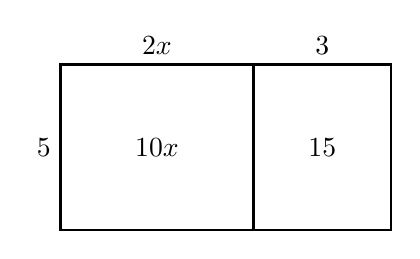
\begin{tikzpicture}[scale=0.7]
  \draw[thick] (0,0) rectangle (6,3);
  \draw[thick] (3.5,0) -- (3.5,3);
  \node[left] at (0,1.5) {$5$};
  \node[above] at (1.75,3) {$2x$};
  \node[above] at (4.75,3) {$3$};
  \node at (1.75,1.5) {$10x$};
  \node at (4.75,1.5) {$15$};
\end{tikzpicture}
\end{center}
\end{questionText}
\choiceA{$5(2x + 3) = 10x + 15$}
\choiceB{$5(2x - 3) = 10x - 15$}
\choiceC{$2(5x + 3) = 10x + 6$}
\choiceD{$3(2x + 5) = 6x + 15$}
\correctAnswer{A}
\explanation{The height is $5$ and the width is split into $2x$ and $3$. Multiply: $5 \times 2x = 10x$ and $5 \times 3 = 15$. So $5(2x + 3) = 10x + 15$.}
\end{practiceQuestion}

\begin{practiceQuestion}{4-3-q23}{gmc}
\begin{questionText}
The area model shows a rectangle split into two parts. What is the expanded form?

\begin{center}
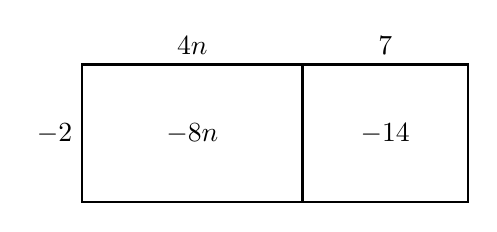
\begin{tikzpicture}[scale=0.7]
  \draw[thick] (0,0) rectangle (7,2.5);
  \draw[thick] (4,0) -- (4,2.5);
  \node[left] at (0,1.25) {$-2$};
  \node[above] at (2,2.5) {$4n$};
  \node[above] at (5.5,2.5) {$7$};
  \node at (2,1.25) {$-8n$};
  \node at (5.5,1.25) {$-14$};
\end{tikzpicture}
\end{center}
\end{questionText}
\choiceA{$-2(4n + 7) = -8n + 14$}
\choiceB{$-2(4n + 7) = -8n - 14$}
\choiceC{$-2(4n - 7) = -8n + 14$}
\choiceD{$2(4n + 7) = 8n + 14$}
\correctAnswer{B}
\explanation{The height is $-2$ and the width splits into $4n$ and $7$. Products: $-2 \times 4n = -8n$ and $-2 \times 7 = -14$. So $-2(4n + 7) = -8n - 14$.}
\end{practiceQuestion}

\begin{practiceQuestion}{4-3-q24}{gmc}
\begin{questionText}
Four students each receive a folder with $x$ worksheets and $5$ pencils. The diagram below shows the total supplies. Which expression represents the total number of items?

\begin{center}
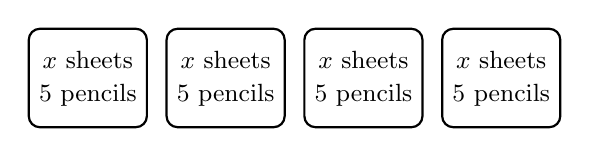
\begin{tikzpicture}[scale=0.5]
  \foreach \i in {0,...,3} {
    \draw[thick, rounded corners] (\i*3.5,0) rectangle (\i*3.5+3,2.5);
    \node[font=\small] at (\i*3.5+1.5,1.7) {$x$ sheets};
    \node[font=\small] at (\i*3.5+1.5,0.8) {$5$ pencils};
  }
\end{tikzpicture}
\end{center}
\end{questionText}
\choiceA{$4x + 5$}
\choiceB{$x + 20$}
\choiceC{$4(x + 5) = 4x + 20$}
\choiceD{$4x + 5 + 5 + 5 + 5 = 4x + 5$}
\correctAnswer{C}
\explanation{Each folder has $x + 5$ items. With $4$ folders: $4(x + 5) = 4x + 20$ total items.}
\end{practiceQuestion}

% --- Graphical Short Answer Questions (3) ---

\begin{practiceQuestion}{4-3-q25}{gsa}
\begin{questionText}
Use the area model to expand $3(4x + 5)$. Fill in the missing values and write the expanded expression.

\begin{center}
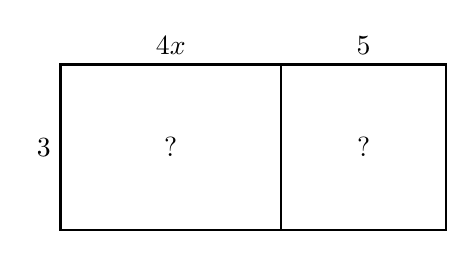
\begin{tikzpicture}[scale=0.7]
  \draw[thick] (0,0) rectangle (7,3);
  \draw[thick] (4,0) -- (4,3);
  \node[left] at (0,1.5) {$3$};
  \node[above] at (2,3) {$4x$};
  \node[above] at (5.5,3) {$5$};
  \node at (2,1.5) {?};
  \node at (5.5,1.5) {?};
\end{tikzpicture}
\end{center}
\end{questionText}
\correctAnswer{$12x + 15$}
\explanation{The left section: $3 \times 4x = 12x$. The right section: $3 \times 5 = 15$. Expanded: $3(4x + 5) = 12x + 15$.}
\end{practiceQuestion}

\begin{practiceQuestion}{4-3-q26}{gsa}
\begin{questionText}
The diagram shows two rectangular flower beds side by side. Both have a width of $4$ feet. Write a simplified expression for the total area.

\begin{center}
\begin{tikzpicture}[scale=0.7]
  % Rectangle 1
  \draw[thick, fill=funGreen!15] (0,0) rectangle (4,3);
  \node[below] at (2,0) {$3x + 2$};
  \node[left] at (0,1.5) {$4$};
  % Rectangle 2
  \draw[thick, fill=funGreen!15] (5,0) rectangle (9,3);
  \node[below] at (7,0) {$x - 1$};
  \node[right] at (9,1.5) {$4$};
\end{tikzpicture}
\end{center}
\end{questionText}
\correctAnswer{$16x + 4$}
\explanation{Area of bed 1: $4(3x + 2) = 12x + 8$. Area of bed 2: $4(x - 1) = 4x - 4$. Total: $12x + 8 + 4x - 4 = 16x + 4$.}
\end{practiceQuestion}

\begin{practiceQuestion}{4-3-q27}{gsa}
\begin{questionText}
The area model below has a missing dimension. Find the value of the missing dimension and write the complete factored and expanded forms.

\begin{center}
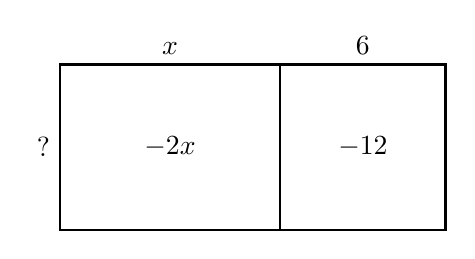
\begin{tikzpicture}[scale=0.7]
  \draw[thick] (0,0) rectangle (7,3);
  \draw[thick] (4,0) -- (4,3);
  \node[left] at (0,1.5) {?};
  \node[above] at (2,3) {$x$};
  \node[above] at (5.5,3) {$6$};
  \node at (2,1.5) {$-2x$};
  \node at (5.5,1.5) {$-12$};
\end{tikzpicture}
\end{center}
\end{questionText}
\correctAnswer{Missing dimension is $-2$; $-2(x + 6) = -2x - 12$}
\explanation{$? \times x = -2x$, so the missing dimension is $-2$. Check: $-2 \times 6 = -12$ \checkmark. Factored: $-2(x + 6)$. Expanded: $-2x - 12$.}
\end{practiceQuestion}
